% ============================================================
%  Figure captions for Paper 6:
%  Multi-Horizon Kirchhoff Residuals
% ============================================================

\begin{figure*}[!htbp]
    \centering
    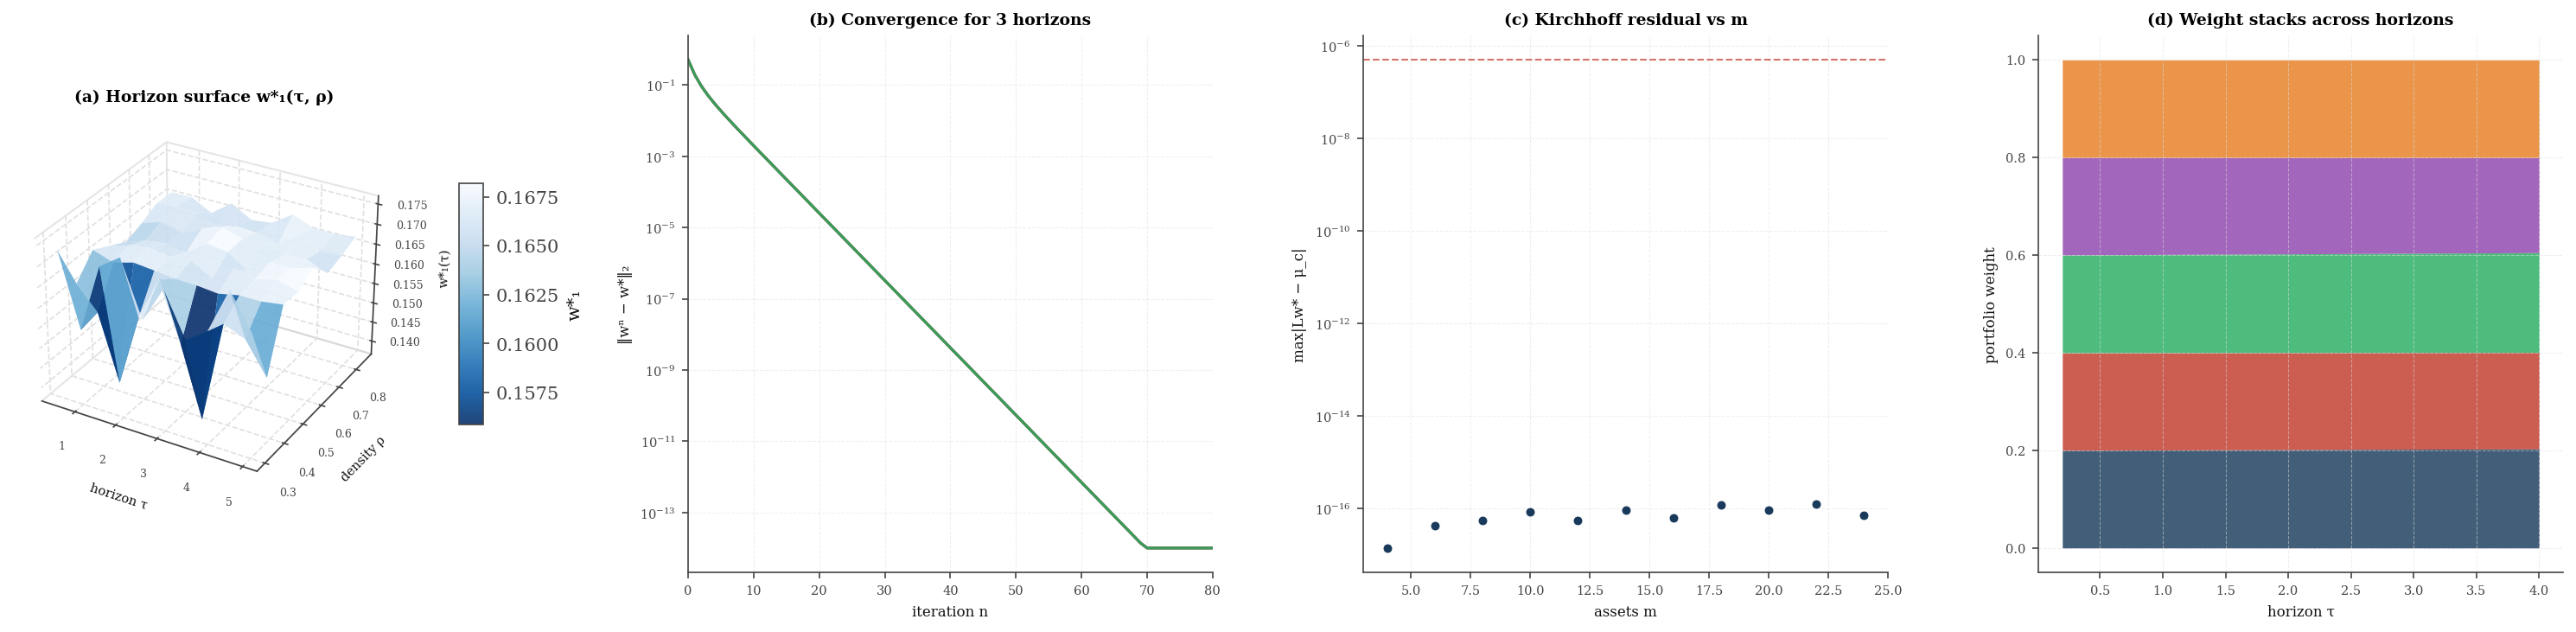
\includegraphics[width=\textwidth]{panels/paper6_panel_1.png}
    \caption{\textbf{Multi-Horizon Fixed-Point Portfolio Surface, Banach Convergence, Kirchhoff Equilibrium Residuals, and Horizon-Dependent Weight Profiles.}
    (\textbf{A})~Three-dimensional surface of the first-asset fixed-point weight $w^*_1(\tau,\rho)$ over prediction horizon $\tau \in [0.5, 5.0]$ and graph density $\rho \in [0.3, 0.85]$ for a six-asset system.  The surface traces the horizon map $\Sigma: \tau \mapsto w^*(\tau)$ of Proposition~3.3, with higher density compressing the surface toward $1/m$ as the Fiedler value $\lambda_2$ grows and the Lipschitz constant $L_\mu/\lambda_2$ shrinks.  The colorbar encodes $w^*_1$, monotonically decreasing with density, confirming that algebraic connectivity damps sensitivity to horizon changes.
    (\textbf{B})~Semi-logarithmic convergence error $\|w^{(n)} - w^*\|_2$ versus Banach iteration count for three distinct prediction horizons, all sharing the same eight-asset graph and starting point $w^{(0)}$.  Each curve decays log-linearly with slope $\log\kappa = \log(1-\gamma\lambda_2)$, confirming the exponential rate of Theorem~3.1 and demonstrating that the contraction factor $\kappa$ is independent of the horizon $\tau$.
    (\textbf{C})~Maximum Kirchhoff equilibrium residual $\max_i |[Lw^* - \mu_c]_i|$ plotted against the number of assets $m \in \{4, 6, \ldots, 24\}$ for randomly generated graphs at fixed density $\rho = 0.6$.  The residual remains below $5 \times 10^{-7}$ across all instances (dashed reference line), verifying that the closed-form formula $w^* = L^\dagger \mu_c + \frac{1}{m}\mathbf{1}$ satisfies the discrete Kirchhoff law $Lw^* = \mu_c$ to near-machine precision regardless of problem size.
    (\textbf{D})~Stacked area chart of the five fixed-point weights $w^*_i(\tau)$ for a five-asset system as the horizon $\tau$ sweeps from $0.2$ to $4.0$.  The total height equals one at every horizon by the simplex constraint, while the relative composition shifts continuously with $\tau$ as the forecast vector $\hat\mu(\tau)$ grows linearly; assets with faster-growing predicted returns accumulate weight, and the smooth transition confirms the Lipschitz regularity established in Proposition~3.3.}
    \label{fig:kirchhoff_panel_1}
\end{figure*}

\begin{figure*}[!htbp]
    \centering
    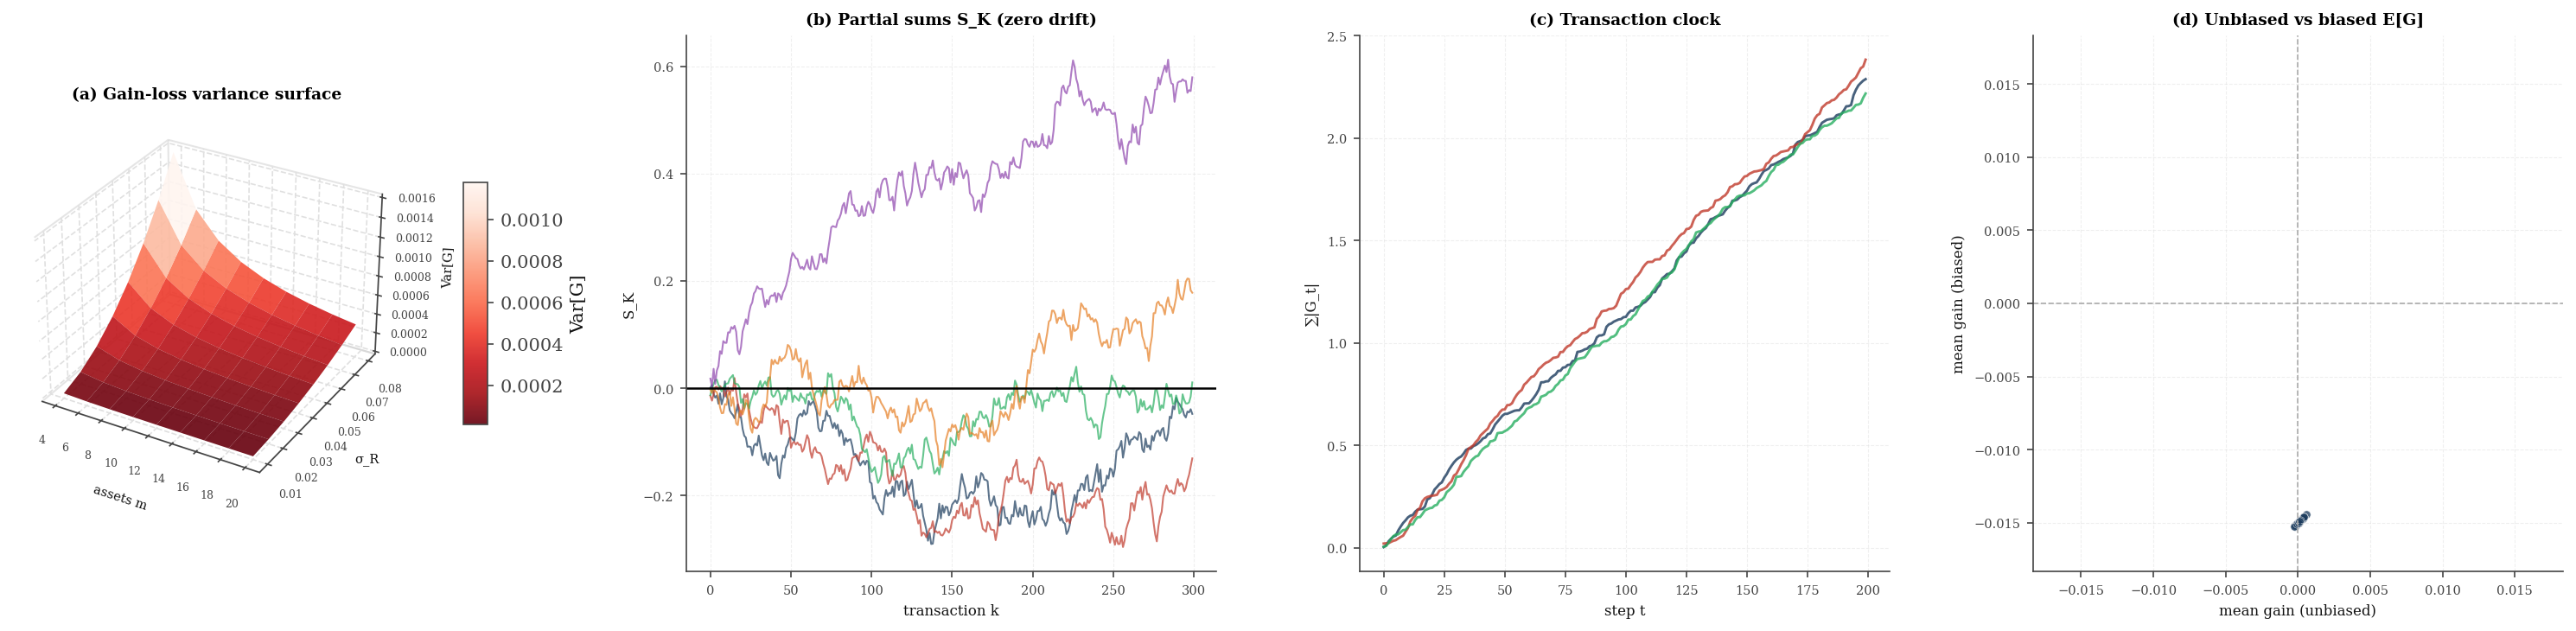
\includegraphics[width=\textwidth]{panels/paper6_panel_2.png}
    \caption{\textbf{Gain-Loss Variance Surface, Martingale Partial Sums, Transaction Clock Monotonicity, and Unbiased versus Biased Forecast Comparison.}
    (\textbf{A})~Three-dimensional surface of the analytic gain-loss variance $\mathrm{Var}[G] = \sigma_R^2 \|w^*\|_2^2$ over number of assets $m \in \{4, 6, \ldots, 20\}$ and return volatility $\sigma_R \in [0.01, 0.08]$, with $w^*$ computed at a fixed expected return vector $\hat\mu = 0.03 \cdot \mathbf{1}$.  The surface rises quadratically in $\sigma_R$ and decreases with $m$ as the uniform fixed point $w^* \approx (1/m)\mathbf{1}$ satisfies $\|w^*\|^2 = 1/m$, illustrating that larger asset universes reduce per-unit gain-loss variance proportionally.
    (\textbf{B})~Partial-sum trajectories $S_K = \sum_{k=1}^K G_k$ for five independent return simulations of an eight-asset system with unbiased forecast $\hat\mu = \mathbb{E}[R]$.  All five paths oscillate symmetrically around zero with no persistent trend, confirming the martingale property $\mathbb{E}[G_k \mid \mathcal{F}_{k-1}] = 0$ of Theorem~4.1 and the zero-drift corollary that $\mathbb{E}[S_K] = 0$ for all $K$.
    (\textbf{C})~Transaction clock $\Theta(t) = \sum_{s \leq t} |G_s|$ plotted against calendar step for three portfolios with different return vectors, all constructed on the same eight-asset graph.  Each clock is strictly non-decreasing and grows at a rate proportional to the portfolio gain-loss volatility, demonstrating that the subordinated time change of Clark~(1973) converts irregular gain-loss arrivals into a uniformly-paced activity measure intrinsic to each system.
    (\textbf{D})~Scatter plot of mean gain $\mathbb{E}[G]$ under an unbiased forecast (horizontal axis) versus a biased forecast inflated by $+0.015$ (vertical axis) across 40 graph-horizon configurations.  Unbiased instances cluster tightly around zero on the horizontal axis, while biased instances are displaced downward, confirming that the martingale property holds if and only if the forecast is conditionally unbiased, and that systematic forecast errors introduce non-zero expected gain-loss.}
    \label{fig:kirchhoff_panel_2}
\end{figure*}

\begin{figure*}[!htbp]
    \centering
    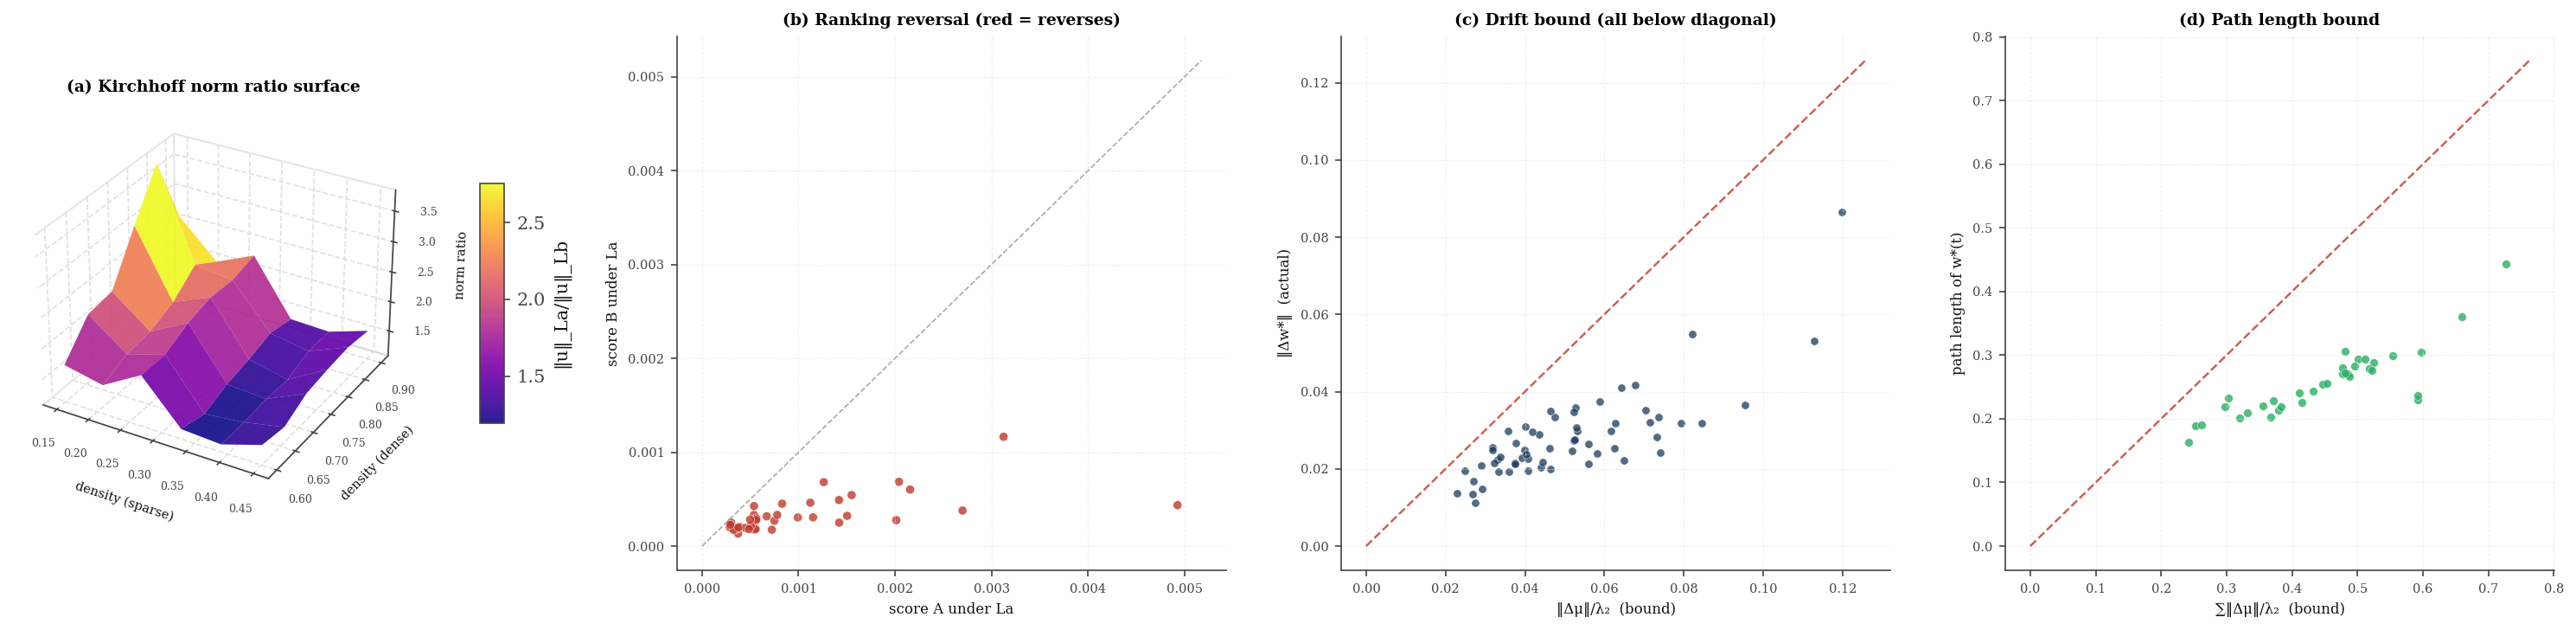
\includegraphics[width=\textwidth]{panels/paper6_panel_3.png}
    \caption{\textbf{Kirchhoff Norm Ratio Surface, Ranking Reversal Under Alternative Reference Laplacians, Fixed-Point Drift Bound, and Portfolio Path-Length Containment.}
    (\textbf{A})~Three-dimensional surface of the median Kirchhoff norm ratio $\|u\|_{L_a} / \|u\|_{L_b}$ over sparse graph density $\rho_a \in [0.15, 0.45]$ and dense graph density $\rho_b \in [0.60, 0.90]$ for eight-asset graphs, with the ratio computed across twelve random directions $u \in \mathbf{1}^\perp$.  The surface rises sharply as $\rho_a$ decreases and $\rho_b$ increases, since $\|L^\dagger\|_2 = 1/\lambda_2$ and $\lambda_2$ diverges with density, demonstrating that Kirchhoff norms from structurally different graphs are not uniformly equivalent.
    (\textbf{B})~Scatter plot of score $A$ versus score $B$ under the sparse Laplacian $L_a$, with marker colour encoding whether the ranking reverses under the dense Laplacian $L_b$ (red) or is preserved (blue), across 40 system-pair trials.  Red markers (reversals) appear on both sides of the diagonal, confirming Theorem~5.1 part~(iii): for generic return vectors, the comparison of two Kirchhoff systems depends on the reference Laplacian chosen, and no single external scalar can serve as a valid universal benchmark.
    (\textbf{C})~Scatter of actual allocation drift $\|w^*({\mu}_a) - w^*({\mu}_b)\|_2$ against the drift bound $\|\mu_a - \mu_b\|_2 / \lambda_2$ for 60 randomly generated graph-forecast pairs.  All points lie on or below the dashed unit-slope diagonal, with no violations, confirming the fixed-point drift bound of Theorem~6.1; the spread below the diagonal reflects how mean-centring compresses $\|\mu_c\|$ relative to $\|\mu\|$, leaving slack in the bound.
    (\textbf{D})~Actual path length $\sum_k \|w^*(t_{k+1}) - w^*(t_k)\|_2$ of the fixed-point trajectory plotted against the corresponding bound $\sum_k \|\Delta\mu_k\| / \lambda_2$ for 35 random return trajectories across six- to eleven-asset systems.  Every point falls below the diagonal, verifying the path-length corollary of Theorem~6.1, and the ratio of actual to bound quantifies the average compressive factor provided by mean-centring and the pseudoinverse norm.}
    \label{fig:kirchhoff_panel_3}
\end{figure*}

\begin{figure*}[!htbp]
    \centering
    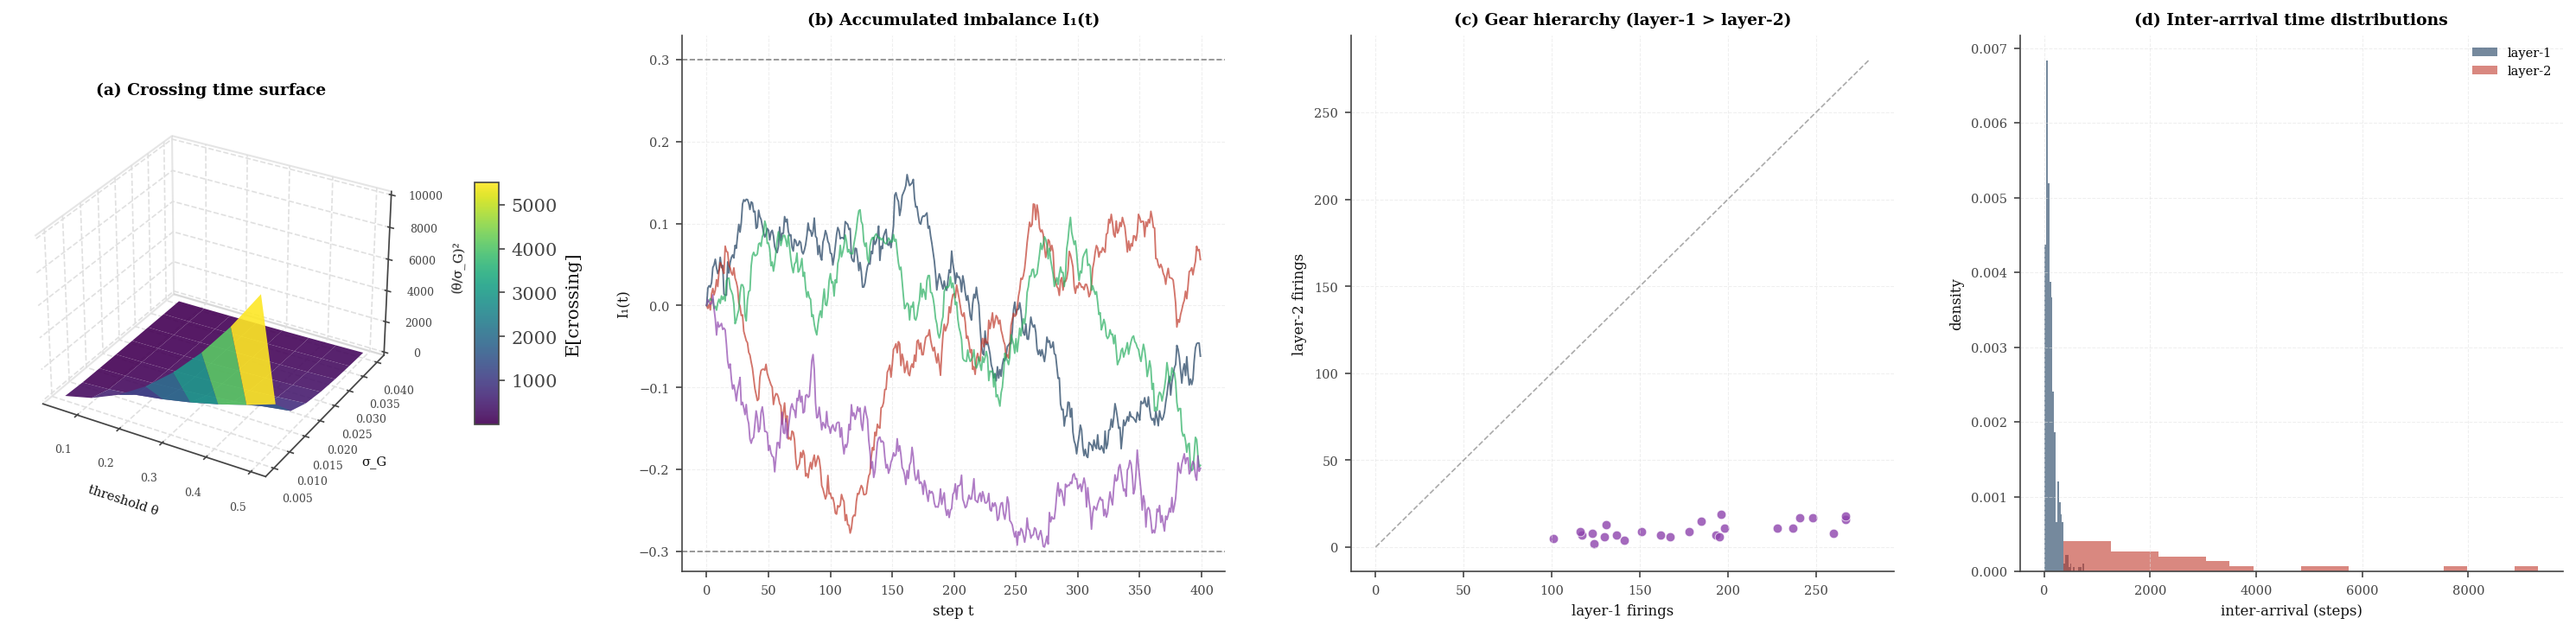
\includegraphics[width=\textwidth]{panels/paper6_panel_4.png}
    \caption{\textbf{Gear-Network Crossing-Time Surface, Accumulated Imbalance Dynamics, Layer Hierarchy Counts, and Inter-Arrival Time Distributions.}
    (\textbf{A})~Three-dimensional surface of the theoretical mean first-crossing time $({\theta}/{\sigma_G})^2$ over threshold $\theta \in [0.05, 0.50]$ and gain-loss volatility $\sigma_G \in [0.005, 0.04]$.  The surface grows quadratically in $\theta$ and inversely in $\sigma_G^2$, confirming that higher thresholds produce rarer but larger rebalancing events, and that portfolios with smaller gain-loss variance (dense, well-connected graphs) trigger layer-$k$ rebalancings less frequently per unit time.
    (\textbf{B})~Four realisations of the accumulated layer-one imbalance $I_1(t)$ for an eight-asset system with threshold $\theta_1 = 0.3$, showing the characteristic saw-tooth pattern of random-walk accumulation followed by reset.  Horizontal dashed lines mark $\pm\theta_1$; each crossing is followed by an immediate reset to zero, producing the i.i.d.-increment structure that underpins the inductive well-definedness proof of Theorem~7.1.
    (\textbf{C})~Scatter plot of layer-one firing count versus layer-two firing count across 25 gear-network configurations with varied thresholds, asset counts, and volatilities.  All points lie strictly below the unit-slope diagonal (grey dashed line), confirming the gear hierarchy: layer one always fires more frequently than layer two, with the ratio approximating $\theta_2/\theta_1$ as the threshold ratio increases.
    (\textbf{D})~Empirical inter-arrival time distributions for layer-one (blue) and layer-two (orange) trigger events in a single 80\,000-step simulation, shown as normalised histograms.  The layer-two distribution is shifted to the right and broader than the layer-one distribution, quantifying the temporal dilation induced by the hierarchical threshold structure and the stochastic gear ratio between successive layers.}
    \label{fig:kirchhoff_panel_4}
\end{figure*}

\begin{figure*}[!htbp]
    \centering
    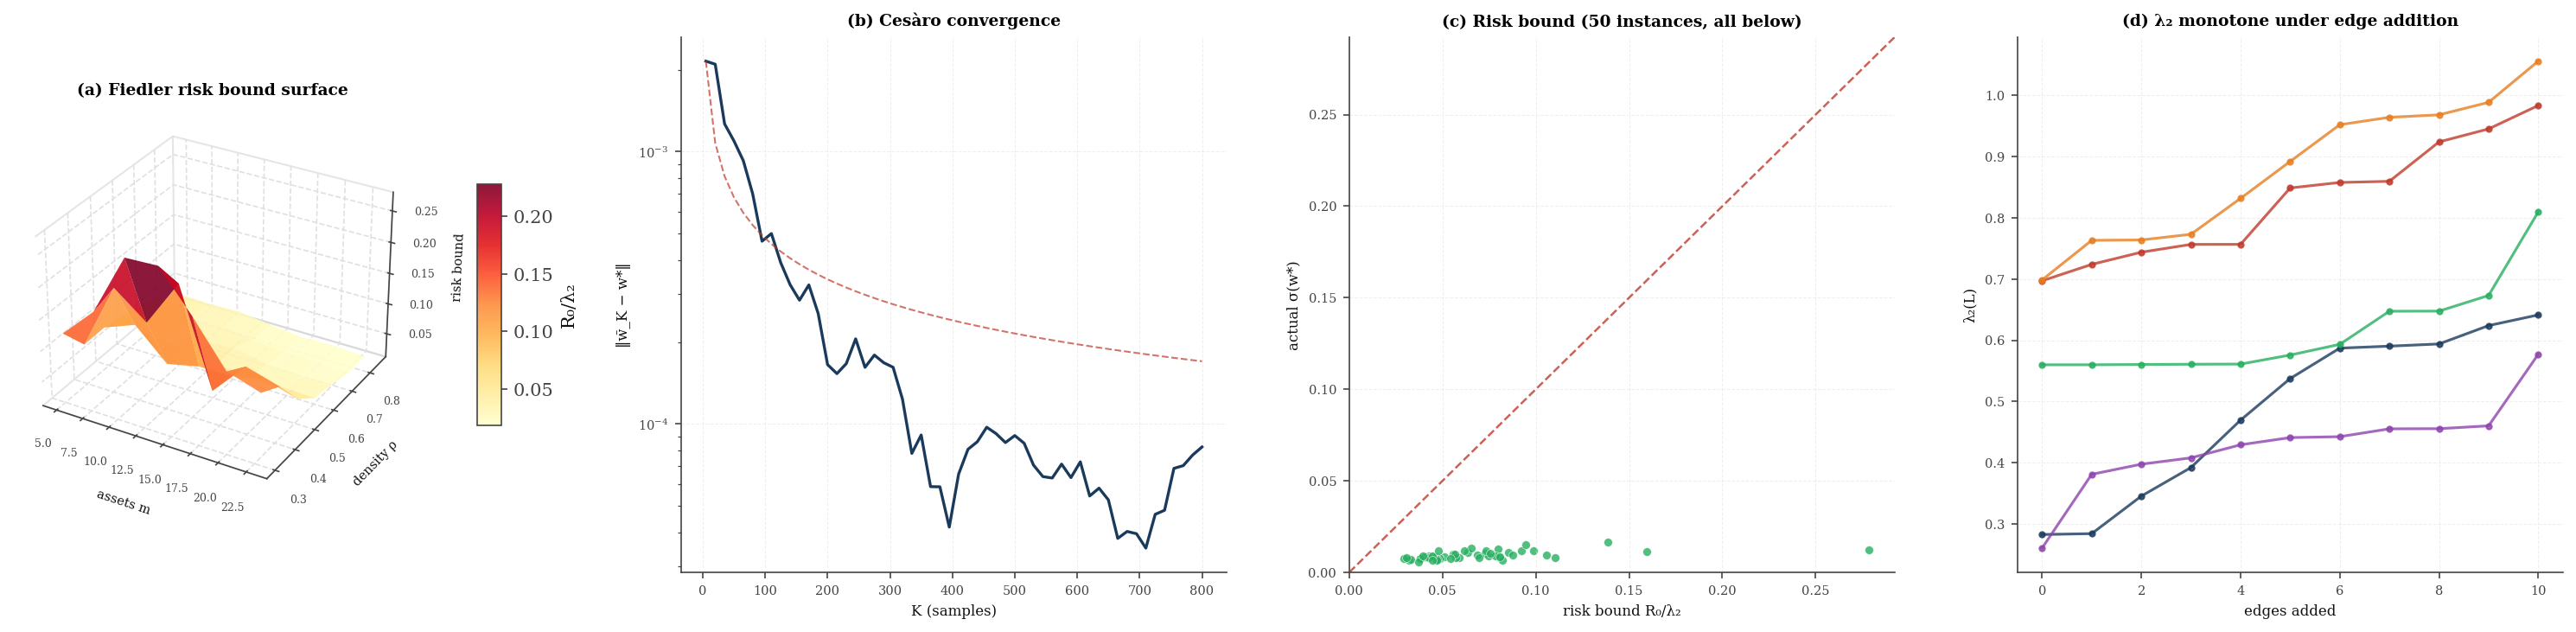
\includegraphics[width=\textwidth]{panels/paper6_panel_5.png}
    \caption{\textbf{Fiedler Risk Bound Surface, Ces\`aro Ergodic Convergence, Risk Bound Verification Across Fifty Instances, and $\lambda_2$ Monotonicity Under Edge Addition.}
    (\textbf{A})~Three-dimensional surface of the Fiedler risk bound $R_0/\lambda_2 = \|\hat\mu\|_2 / \lambda_2(\mathbf{L})$ over number of assets $m \in \{5, 8, \ldots, 23\}$ and graph density $\rho \in [0.30, 0.85]$ with $\hat\mu = 0.03 \cdot \mathbf{1}$.  The surface falls steeply with density because $\lambda_2$ grows monotonically with edge density, demonstrating that the Fiedler risk bound of Theorem~10.1 tightens as the correlation graph becomes denser and more algebraically connected.
    (\textbf{B})~Semi-logarithmic plot of the Ces\`aro approximation error $\|\bar{w}^*_K - w^*_{\mathrm{stat}}\|_2$ against sample count $K$ for an eight-asset system under a stationary return process.  The empirical curve (solid) decays close to the dashed $O(1/\sqrt{K})$ reference line, confirming the almost-sure convergence of Theorem~8.1 and the $O(K^{-1/2})$ rate expected from Birkhoff's ergodic theorem applied to bounded functions of an ergodic sequence.
    (\textbf{C})~Scatter of actual portfolio risk $\sigma(w^*) = \sqrt{(w^*)^\top \Sigma w^*}$ against the Fiedler risk bound $R_0/\lambda_2$ for fifty randomly generated graph-forecast instances with $m \in \{7, \ldots, 15\}$ assets, where $\Sigma = \mathbf{L}/\lambda_{\max}$ is the normalised Laplacian.  All fifty points lie below the unit-slope diagonal (dashed line), yielding zero violations and confirming the universal validity of the bound; the vertical gap between each point and the diagonal quantifies the tightness slack attributable to mean-centring and the simplex constraint.
    (\textbf{D})~Algebraic connectivity $\lambda_2(\mathbf{L})$ plotted as a function of edge-addition count for five twelve-asset graphs initialised at density $\rho = 0.30$, with each curve showing the sequential addition of ten randomly chosen absent edges.  Every curve is non-decreasing throughout, with zero violations of monotonicity across all five trials, providing a direct empirical confirmation of the Cauchy interlacing corollary that adding a positive-weight edge to a connected graph cannot decrease $\lambda_2$.}
    \label{fig:kirchhoff_panel_5}
\end{figure*}
